\chapter{流形上的映射}
\label{chap:manifold-maps}

把地球仪绕地轴转过一个角度，每个城市都移到了新的位置；在球面上画一条航线，就是把时间区间映到球面上。这两件事都是流形之间的映射。映射首先对应点：给定原来的点，找到它被送到哪里。但我们还关心更多：经过一点的运动方向被转到哪个方向，速度是否被拉伸，一个方向上的读数怎样随映射换算。这些问题的答案不在点的对应本身，而在映射的微分中。

本章沿“点—方向—读数”的顺序展开。第~\ref{sec:mmaps-smooth-maps}节用两侧的坐标图定义流形之间的光滑映射，区分同一点的坐标改写与把点实际移到另一点，并把第~\ref{chap:manifold-basics}章的曲线和函数看作特例。第~\ref{sec:mmaps-differentials}节由曲线速度的推送得到切空间之间的线性映射，再考察对整个向量场逐点推送时会遇到的困难：一般映射的推送结果未必在目标上构成向量场。

第~\ref{sec:mmaps-pullback}节转向余切向量。读数的换算方向与切向量相反，从目标点拉回到原像点；正因为方向相反，协向量场的拉回对任何光滑映射都有定义，不受推送向量场时遇到的限制。拉回与函数微分的关系$\mathrm d(f\circ F)=F^*(\mathrm df)$把两个方向的运算联系起来。

本章只处理给定映射的局部操作。用映射判断两个流形是否在光滑意义下等价、一个流形能否作为另一个流形的子流形，需要整体的可逆性与拓扑条件，这是第~\ref{chap:manifold-relations}章的任务；一般微分形式的拉回在第~\ref{chap:manifold-calculus}章定义交替形式之后推广。

\section{光滑映射}
\label{sec:mmaps-smooth-maps}

设$M$是$m$维光滑流形，$N$是$n$维光滑流形，$F:M\to N$是映射。判断$F$是否光滑，仍要借助坐标，但现在两侧都要用图：输入的点用$M$的图记录，输出的点用$N$的图记录。这样得到的是欧氏开集之间的映射，可以用多元微积分检查。

\paragraph{坐标表示与光滑性}
设$(U,\varphi)$是$M$的图，$(V,\psi)$是$N$的图，并且$F(U)\subseteq V$。把输入坐标先送回点，作用$F$，再读出输出坐标，得到
\begin{equation}
\hat F=\psi\circ F\circ\varphi^{-1}:\varphi(U)\to\psi(V)\subseteq\mathbb R^n ,
\label{eq:mmaps-coordinate-representation}
\end{equation}
称为$F$在这对图下的\term{坐标表示}（coordinate representation）。条件$F(U)\subseteq V$保证输出点能用同一张图$\psi$读出。

\begin{definition}[光滑映射]
\label{def:mmaps-smooth-map}
映射$F:M\to N$称为\term{光滑映射}（smooth map），若$F$连续，并且对每个$p\in M$，存在包含$p$的图$(U,\varphi)$与包含$F(p)$的图$(V,\psi)$，使$F(U)\subseteq V$且坐标表示\eqref{eq:mmaps-coordinate-representation}光滑。$M$或$N$带边界时，光滑性按第~\ref{chap:manifold-basics}章的约定理解：半空间开子集上的映射光滑，指它在每点附近能光滑延拓到一个欧氏开邻域上。
\end{definition}

连续性的作用是保证满足$F(U)\subseteq V$的图存在：任给包含$F(p)$的图$(V,\psi)$，$F^{-1}(V)$是包含$p$的开集，把$M$的图限制到$U\cap F^{-1}(V)$上即可。

\paragraph{与图的选择无关}
定义只要求每点附近存在一对图使坐标表示光滑。换用别的图对，结论不变：若$(U',\varphi')$与$(V',\psi')$是另一对满足条件的图，在重叠处
\[
\psi'\circ F\circ\varphi'^{-1}=(\psi'\circ\psi^{-1})\circ\hat F\circ(\varphi\circ\varphi'^{-1}),
\]
右端是两个光滑坐标变换与$\hat F$的复合，仍光滑。同样的论证说明光滑映射的复合仍是光滑映射：若$F:M\to N$与$G:N\to P$都光滑，则在合适的图下$\widehat{G\circ F}=\hat G\circ\hat F$，光滑映射的复合光滑。

\paragraph{特例：曲线与函数}
第~\ref{chap:manifold-basics}章的两类对象都是光滑映射的特例。把区间$I$看作一维流形（带端点时为带边界流形），用恒等映射作图，光滑曲线$\gamma:I\to M$就是$I$到$M$的光滑映射，坐标表示是坐标曲线$\varphi\circ\gamma$。把$\mathbb R$看作一维流形，光滑函数$f:M\to\mathbb R$就是$M$到$\mathbb R$的光滑映射，坐标表示是$\hat f=f\circ\varphi^{-1}$。今后关于一般光滑映射的结论，都可以用这两类特例检验。

\paragraph{例子：球面的旋转}
设$\bm R(\theta)$是平面上转角为$\theta$的旋转矩阵。绕竖直轴转$\theta$的映射
\[
R_\theta:S^2\to S^2,\qquad R_\theta(\bm y)=(\bm R(\theta)(y_1,y_2)^\top,\;y_3)
\]
把球面送到自身。在北极图中，$\sigma_N(R_\theta(\bm y))=\bm R(\theta)(y_1,y_2)^\top/(1-y_3)=\bm R(\theta)\sigma_N(\bm y)$，所以坐标表示是线性映射$\hat R_\theta(\bm u)=\bm R(\theta)\bm u$，光滑。北极是$R_\theta$的不动点，那里改用南极图，坐标表示同样是$\bm w\mapsto\bm R(\theta)\bm w$。于是$R_\theta$是光滑映射。

绕水平轴的旋转会把北极移走，这时需要按点选择图。例如绕$y_1$轴转$\pi/2$的映射$Q(\bm y)=(y_1,-y_3,y_2)$把北极送到$(0,-1,0)$，把点$(0,1,0)$送到北极。在$(0,1,0)$附近，输入可以用北极图，输出却必须用南极图，因为北极不在北极图的定义域内。定义中“对每个$p$存在一对图”正是为这种情况准备的。

\paragraph{改写坐标与移动点}
同一个计算式可以表示两件不同的事。取$p=(0,\tfrac35,\tfrac45)$，北极图坐标为$(0,3)$。旋转$R_\theta$把$p$送到$(-\tfrac35\sin\theta,\tfrac35\cos\theta,\tfrac45)$，坐标变为$(-3\sin\theta,3\cos\theta)$：点真的移动了，坐标的变化反映了这一移动。坐标变换$\tau=\sigma_S\circ\sigma_N^{-1}$把$(0,3)$变为$(0,\tfrac13)$，点却没有动，只是换了一张图来记录。

用本节的语言说，坐标变换是恒等映射$\mathrm{id}:S^2\to S^2$在输入用$\sigma_N$、输出用$\sigma_S$时的坐标表示。所以判断一个坐标公式描述的是什么，不能只看公式，还要看它是同一映射在不同图下的表示，还是不同映射在同一图下的表示。前者改变的是记录，后者改变的是点；后文讨论微分时，前者只改变切向量的分量，后者把切向量送到另一个点的切空间。

\section{映射的微分}
\label{sec:mmaps-differentials}

点被映射移动时，经过它的运动也跟着改变。地球仪转过一个角度，沿一条经线向北的航线被转到另一条经线上，航线上每点的运动方向也都被带到了别处。本节先对单个切向量回答“方向被送到哪里”，得到切空间之间的线性映射；再对整个向量场逐点执行这一操作，看结果能否在目标流形上构成向量场。

前者对任何光滑映射都成立，后者却需要映射满足额外条件。两者的差别，就是下一节拉回运算的出发点。

\subsection{切向量的推送}
\label{sec:mmaps-tangent-pushforward}

\paragraph{由曲线速度定义}
先回忆欧氏空间的情形。映射$\bm f:\mathbb R^m\to\mathbb R^n$在$\bm x$处的Jacobian矩阵$\bm J$是最佳线性近似：小位移$\bm h$引起的输出变化约为$\bm J\bm h$，详见\BookChapterRef{chap:multivariate-differentiation}{卷二第17章“多元函数微分”}。流形上不能写$p+\bm h$，因为点不能相加，所以要把“小位移”换成“经过$p$的曲线及其速度”。

先在坐标里看这个近似长什么样。对投影的坐标表示\eqref{eq:mmaps-projection-chart}求偏导，第$i$个分量对$u_j$求导，由商的求导法则得到
\[
\frac{\partial\hat\pi_i}{\partial u_j}
=\frac{2\delta_{i,j}}{\rho+1}-\frac{4u_iu_j}{(\rho+1)^2}.
\]
写成矩阵，
\begin{equation}
\bm J_{\hat\pi}(\bm u)=\frac{2}{\rho+1}\bm I-\frac{4}{(\rho+1)^2}\bm u\bm u^\top .
\label{eq:mmaps-projection-jacobian}
\end{equation}

在$\bm u=(0,3)$处，$\rho=9$，$\bm u\bm u^\top=\operatorname{diag}(0,9)$，代入后
\[
\bm J_{\hat\pi}(0,3)=\frac15\bm I-\frac{1}{25}\operatorname{diag}(0,9)
=\operatorname{diag}(0.2,\ -0.16).
\]
验证近似的精度。把$u_2$从$3$改为$3.2$，由式~\eqref{eq:mmaps-projection-chart}，投影的第二个分量从$0.6$变为$6.4/11.24\approx0.5694$，变化量约为$-0.0306$。线性近似给出
\[
-0.16\times0.2=-0.032,
\]
两者只差$0.0014$。

图~\ref{fig:mmaps-linear-approx}把这种近似画成方格的形变：方格越小，弯曲的像越接近平行四边形。微分要提取的就是这个平行四边形所代表的线性映射。

\begin{BookInlineFigure}
  \centering
  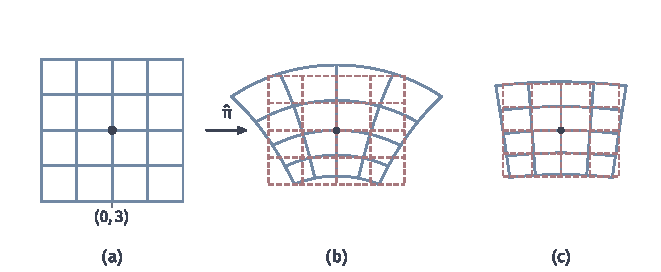
\includegraphics[width=112mm]{figures/04-spaces-measures-and-geometry/04-manifolds/matplotlib/mmaps-linear-approx/figure.pdf}
  \caption{微分是局部线性近似。(a)北极图中以$(0,3)$为心、半边长$0.8$的方格。(b)方格在$\hat\pi$下的像（蓝）与线性映射$\bm J=\operatorname{diag}(0.2,-0.16)$的像（红虚线），二者都按比例放大并平移到同一中心。(c)半边长缩小到$0.2$再放大相应倍数，蓝红两组线几乎重合。}
  \label{fig:mmaps-linear-approx}
\end{BookInlineFigure}

现在在流形上做同样的事。设$F:M\to N$光滑，$p$是内点，$\gamma$是经过$p$的曲线，$\gamma(0)=p$。$F$把它送成经过$F(p)$的曲线$F\circ\gamma$。取一对图，并记$\bm J_{\hat F}$为坐标表示的Jacobian矩阵。由欧氏链式法则，
\begin{equation}
(\psi\circ F\circ\gamma)'(0)=\bm J_{\hat F}(\varphi(p))\,(\varphi\circ\gamma)'(0).
\label{eq:mmaps-velocity-push}
\end{equation}

这个式子说了两件事。右端只依赖$\gamma$在$p$处的坐标速度，所以等价的两条曲线被送成等价的曲线，“把曲线送过去再取速度”是定义在$T_pM$上的操作。右端又是矩阵乘向量，所以这个操作是线性的。图~\ref{fig:mmaps-pushforward-sphere}（见本小节末的例子）是它在球面上的样子。

\begin{definition}[映射的微分]
\label{def:mmaps-differential}
设$F:M\to N$光滑，$p\in M$，$(U,\varphi)$与$(V,\psi)$是定义~\ref{def:mmaps-smooth-map}中的一对图。$F$在$p$处的\term{微分}（differential）是线性映射
\begin{equation}
\mathrm dF_p:T_pM\to T_{F(p)}N,
\label{eq:mmaps-differential}
\end{equation}
它把$p$处在图$\varphi$中分量为$\bm v$的切向量，送到$F(p)$处在图$\psi$中分量为$\bm J_{\hat F}(\varphi(p))\bm v$的切向量。切向量$\mathrm dF_p(\bm v)$称为$\bm v$在$F$下的\term{推送}（pushforward）。
\end{definition}

当$p$与$F(p)$都是内点时，式~\eqref{eq:mmaps-velocity-push}说明定义等价于
\[
\mathrm dF_p([\gamma])=[F\circ\gamma].
\]
这是最直观的理解：把曲线送过去，再取它的切向量。

在坐标基下，定义可以写成
\begin{equation}
\mathrm dF_p\Bigl(\left.\frac{\partial}{\partial x_j}\right|_p\Bigr)
=\sum_{k=1}^n\frac{\partial\hat F_k}{\partial x_j}(\varphi(p))
\left.\frac{\partial}{\partial y_k}\right|_{F(p)},
\label{eq:mmaps-differential-basis}
\end{equation}
其中$y_1,\ldots,y_n$是图$\psi$中的坐标。也就是说，$\mathrm dF_p$在两组坐标基下的矩阵就是坐标表示的Jacobian矩阵，第$j$列记录第$j$个输入基向量被送到哪里。

\paragraph{与图无关}
定义用了一对图，需要检查换图后得到的是同一个线性映射。换用另一对图$(U',\varphi')$与$(V',\psi')$，记坐标变换为$\tau_M=\varphi'\circ\varphi^{-1}$和$\tau_N=\psi'\circ\psi^{-1}$。坐标表示变成
\[
\hat F'=\tau_N\circ\hat F\circ\tau_M^{-1}.
\]

对它用链式法则，各处的Jacobian矩阵取在相应的点上，得到
\begin{equation}
\bm J_{\hat F'}=\bm J_{\tau_N}\,\bm J_{\hat F}\,\bm J_{\tau_M}^{-1}.
\label{eq:mmaps-jacobian-change}
\end{equation}

现在核对两种算法。同一切向量在新图中的分量是$\bm v'=\bm J_{\tau_M}\bm v$，代入式~\eqref{eq:mmaps-jacobian-change}，
\[
\bm J_{\hat F'}\bm v'=\bm J_{\tau_N}\bm J_{\hat F}\bm J_{\tau_M}^{-1}\bm J_{\tau_M}\bm v=\bm J_{\tau_N}(\bm J_{\hat F}\bm v).
\]
左端是用新图算出的输出分量，右端是旧图算出的输出向量换到新图后的分量，两者相等。所以微分是同一个线性映射，改变的只是它的矩阵，这与卷二中线性映射换基时矩阵的变化完全类似。

用旋转$R_{\pi/2}$核对一次。第~\ref{chap:manifold-basics}章给出转移映射$\tau$的Jacobian矩阵
\[
\bm J_\tau(\bm u)=\frac{\rho\bm I-2\bm u\bm u^\top}{\rho^2}.
\]
在$p$处，$\bm u=(0,3)$；在$R_{\pi/2}(p)$处，$\bm u=(-3,0)$。两处$\rho=9$，代入得
\[
\bm J_\tau(0,3)=\operatorname{diag}(\tfrac19,-\tfrac19),\qquad
\bm J_\tau(-3,0)=\operatorname{diag}(-\tfrac19,\tfrac19).
\]

北极图中旋转的矩阵是$\bm R(\tfrac\pi2)$。按式~\eqref{eq:mmaps-jacobian-change}换到南极图，先算右边两个因子，再乘左边的因子：
\[
\bm R(\tfrac\pi2)\operatorname{diag}(9,-9)
=\begin{bmatrix}0&9\\9&0\end{bmatrix},\qquad
\operatorname{diag}(-\tfrac19,\tfrac19)\begin{bmatrix}0&9\\9&0\end{bmatrix}
=\begin{bmatrix}0&-1\\1&0\end{bmatrix}.
\]
结果还是$\bm R(\tfrac\pi2)$，与第~\ref{sec:mmaps-smooth-maps}节在南极图中得到的坐标表示$\bm w\mapsto\bm R(\theta)\bm w$一致。

\paragraph{边界点处的微分}
边界点处，定义里的$\bm J_{\hat F}$要取坐标表示的光滑延拓的Jacobian矩阵。延拓不唯一，需要说明结果不受影响。设$\bm x$是半空间$\mathbb H^m$的边界点，$E_1,E_2$是$\hat F$在$\bm x$附近的两个光滑延拓。

关键在于，$\bm x$处的偏导数只用得到半空间内的函数值。沿边界方向$\bm e_j$（$j<m$）的差商，用到的点$\bm x+h\bm e_j$仍在边界上。沿内法方向$\bm e_m$，极限存在，所以可以只取$h>0$，用到的点$\bm x+h\bm e_m$在半空间内。这些点上$E_1=E_2=\hat F$，所以两个延拓的偏导数相同。

图~\ref{fig:mmaps-boundary-extension}是一维的情形：$[0,\infty)$上的函数$\sin x$有无穷多种光滑延拓，它们在$x<0$的部分可以相差很大，但在$x=0$处的斜率都是右导数$1$。

\begin{BookInlineFigure}
  \centering
  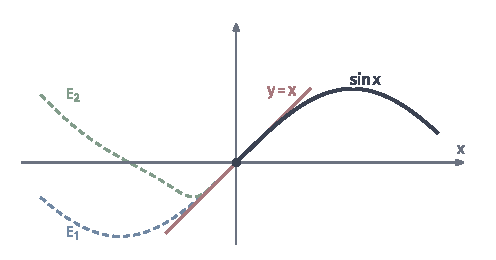
\includegraphics[width=84mm]{figures/04-spaces-measures-and-geometry/04-manifolds/matplotlib/mmaps-boundary-extension/figure.pdf}
  \caption{边界点处的微分与延拓无关。实线是定义在$[0,\infty)$上的$\sin x$；虚线是它在$x<0$处的两个光滑延拓$E_1=\sin x$与$E_2=\sin x+1.6\,e^{-1/x^2}$（$x<0$）。红线是二者在$0$处共同的切线$y=x$。}
  \label{fig:mmaps-boundary-extension}
\end{BookInlineFigure}

\paragraph{链式法则}
复合映射的微分是各步微分的复合。这是欧氏链式法则在流形上的形式，也是流形上做微分计算最常用的工具。

\begin{theorem}[链式法则]
\label{thm:mmaps-chain-rule}
设$F:M\to N$与$G:N\to P$都光滑，$p\in M$。则
\begin{equation}
\mathrm d(G\circ F)_p=\mathrm dG_{F(p)}\circ\mathrm dF_p .
\label{eq:mmaps-chain-rule}
\end{equation}
特别地，$\mathrm d(\mathrm{id}_M)_p$是$T_pM$上的恒等映射。
\end{theorem}

\begin{proof}
按定理~\ref{thm:mmaps-composition}的证明选取三张图，使$F$的输出图与$G$的输入图是同一张$\psi$，这时
\[
\widehat{G\circ F}=\hat G\circ\hat F .
\]
记$\bm x=\varphi(p)$。欧氏链式法则给出
\[
\bm J_{\hat G\circ\hat F}(\bm x)=\bm J_{\hat G}(\hat F(\bm x))\,\bm J_{\hat F}(\bm x).
\]
右端正是$\mathrm dG_{F(p)}$与$\mathrm dF_p$的矩阵之积。边界点处把各坐标表示换成光滑延拓，等式不变。

恒等映射在同一张图下的坐标表示是恒等映射，Jacobian矩阵为单位矩阵，第二个结论随之成立。
\end{proof}

\paragraph{秩}
$\mathrm dF_p$是有限维线性空间之间的线性映射，它有秩。秩说明映射在一点附近保留了多少个独立方向。

\begin{definition}[映射的秩]
\label{def:mmaps-rank}
线性映射$\mathrm dF_p$的秩称为$F$在$p$处的秩，记作$\operatorname{rank}_pF$。在坐标中，它等于$\bm J_{\hat F}(\varphi(p))$的秩。
\end{definition}

由式~\eqref{eq:mmaps-jacobian-change}，换图时矩阵左乘、右乘可逆矩阵，秩不变，所以这个定义与图无关。把它算出来，就知道映射在这一点把多少个方向“压扁”了。

投影$\pi$是最好的例子。式~\eqref{eq:mmaps-projection-jacobian}中，$\bm u\bm u^\top$只在方向$\bm u$上起作用，所以矩阵有两个特征方向。沿$\bm u$的特征值是
\[
\frac{2}{\rho+1}-\frac{4\rho}{(\rho+1)^2}=\frac{2(1-\rho)}{(\rho+1)^2},
\]
与$\bm u$垂直的方向上特征值是$2/(\rho+1)$。

后者永远不为零，前者只在$\rho=1$时为零。$\rho=1$的点正是赤道，因为这时$y_3=(\rho-1)/(\rho+1)=0$。于是$\pi$在赤道上秩为$1$，在其余点秩为$2$；北极不在这张图中，在南极图的原点用同样的公式得到矩阵$2\bm I$，秩也是$2$。

几何上这很合理，图~\ref{fig:mmaps-rank-projection}(a)(b)画出了这件事。赤道上切平面是竖直的，向下投影时其中的竖直方向被压成零，切平面只剩一条线；其余点的切平面只是被斜着压扁，仍然保持二维。

\begin{BookInlineFigure}
  \centering
  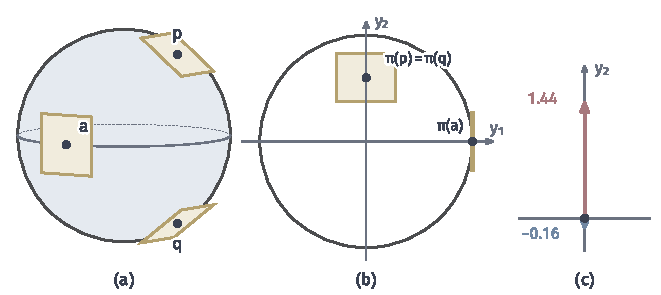
\includegraphics[width=112mm]{figures/04-spaces-measures-and-geometry/04-manifolds/matplotlib/mmaps-rank-projection/figure.pdf}
  \caption{投影$\pi$的秩与多个原像。(a)球面上的三小块切平面（黄），分别在$p=(0,\tfrac35,\tfrac45)$、$q=(0,\tfrac35,-\tfrac45)$与赤道点$a=(1,0,0)$处。(b)$p,q$处的切平面块投影成同一个矩形，秩为$2$；$a$处的切平面块投影成一条线段，秩为$1$。(c)$\partial_{u_2}$在$p$、$q$处的推送都在$\pi(p)$处的切空间中，第二分量分别为$-0.16$（蓝）与$1.44$（红）。}
  \label{fig:mmaps-rank-projection}
\end{BookInlineFigure}

高度函数$h$也可以这样看。它在两极以外秩为$1$，在两极秩为$0$，因为第~\ref{chap:manifold-basics}章已经算出$\mathrm dh_N=0$。可见秩会随点变化，只看一点的秩不能决定映射附近的形状，这个问题在第~\ref{chap:manifold-relations}章展开。

\paragraph{函数与曲线的情形}
第~\ref{chap:manifold-basics}章分别定义过函数的微分和曲线的速度，它们都应当是映射微分的特例，这里核对一下记号确实不冲突。

对光滑函数$f:M\to\mathbb R$，目标在每点$c$处的切空间由一个基向量$\frac{\mathrm d}{\mathrm dt}\big|_c$张成，把$a\,\frac{\mathrm d}{\mathrm dt}\big|_c$等同于实数$a$，就有$T_c\mathbb R=\mathbb R$。在这一等同下，式~\eqref{eq:mmaps-differential-basis}说明
\[
\mathrm df_p(\bm v)=\sum_{j=1}^m\frac{\partial\hat f}{\partial x_j}(\varphi(p))\,v_j ,
\]
这正是第~\ref{chap:manifold-basics}章定义的余切向量$\mathrm df_p$对切向量的读数。

对光滑曲线$\gamma:I\to M$，曲线的速度就是参数区间上单位切向量的推送：
\[
\gamma'(t_0)=\mathrm d\gamma_{t_0}\Bigl(\left.\frac{\mathrm d}{\mathrm dt}\right|_{t_0}\Bigr).
\]
于是链式法则\eqref{eq:mmaps-chain-rule}用到$F\circ\gamma$上，就得到前面“把曲线送过去再取速度”的公式：
\[
(F\circ\gamma)'(t_0)=\mathrm dF_{\gamma(t_0)}(\gamma'(t_0)).
\]

\paragraph{例子：旋转与高度函数}
旋转$R_\theta$在北极图中的坐标表示是线性映射$\bm R(\theta)$，线性映射的Jacobian矩阵就是它自己，所以微分在坐标基下的矩阵也是$\bm R(\theta)$。取$p=(0,\tfrac35,\tfrac45)$，把$\bm e_1$代入，得到
\[
\mathrm d(R_\theta)_p\bigl(\partial_{u_1}|_p\bigr)
=\cos\theta\,\partial_{u_1}|_{R_\theta(p)}+\sin\theta\,\partial_{u_2}|_{R_\theta(p)} .
\]
输入向量属于$T_pS^2$，输出向量属于$T_{R_\theta(p)}S^2$，是另一个点的切空间。$\bm R(\theta)$可逆，所以$R_\theta$在每点的秩都是$2$。

取$\theta=\pi/2$，上式变成
\[
\mathrm d(R_{\pi/2})_p(\partial_{u_1}|_p)=\partial_{u_2}|_{R_{\pi/2}(p)} .
\]
在$\mathbb R^3$中看一下这个结果是否合理。第~\ref{chap:manifold-basics}章算出$\partial_{u_1}|_p$的样子是$(\tfrac15,0,0)$，绕竖直轴转$\pi/2$后变成$(0,\tfrac15,0)$。

另一方面，对$\sigma_N^{-1}$关于$u_2$在$(-3,0)$处求导，第二个分量的导数是
\[
\frac{2(\rho+1)-4u_2^2}{(\rho+1)^2}=\frac{20}{100}=\frac15,
\]
其余两个分量含因子$u_2$，导数为零。所以$\partial_{u_2}|_{R_{\pi/2}(p)}=(0,\tfrac15,0)$，两边一致。图~\ref{fig:mmaps-pushforward-sphere}画的就是这组数据。

\begin{BookInlineFigure}
  \centering
  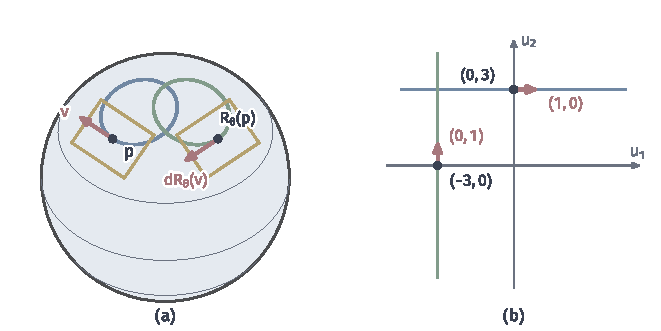
\includegraphics[width=112mm]{figures/04-spaces-measures-and-geometry/04-manifolds/matplotlib/mmaps-pushforward-sphere/figure.pdf}
  \caption{切向量的推送。(a)球面上，经过$p$的蓝色曲线$\gamma(t)=\sigma_N^{-1}(t,3)$被$R_\theta$（$\theta=\pi/2$）转成经过$R_\theta(p)$的绿色曲线，黄色平行四边形是两点处的切平面，红箭头是速度$\bm v=\partial_{u_1}|_p$及其推送，长度按实际放大$2$倍。(b)北极图中，两条曲线分别是直线$u_2=3$与$u_1=-3$，速度分量从$(1,0)$变为$(0,1)$。}
  \label{fig:mmaps-pushforward-sphere}
\end{BookInlineFigure}

旋转$Q$可以检验换图的情形。对式~\eqref{eq:mmaps-horizontal-rotation}在$\bm u=(0,1)$处求偏导。记分母为$D=\rho+1+2u_2$，此处$D=4$，$\partial_{u_1}D=0$，$\partial_{u_2}D=4$，第二个分子$1-\rho$在此处为零，于是
\[
\bm J_{\hat Q}(0,1)=\begin{bmatrix}2/D&0\\0&-2u_2/D\end{bmatrix}
=\operatorname{diag}(\tfrac12,\ -\tfrac12).
\]

在$\mathbb R^3$中验证第一列。$\partial_{u_1}|_a$是向量$(1,0,0)$，$Q$不改变第一个分量，推送后仍是$(1,0,0)$。南极图在原点处$\partial_{w_1}|_N=(2,0,0)$，所以结果是$\tfrac12\partial_{w_1}$，与矩阵的第一列一致。

第二列同理。$\partial_{u_2}|_a=(0,0,1)$，被$Q$送到$(0,-1,0)$；$\partial_{w_2}|_N=(0,2,0)$，所以结果是$-\tfrac12\partial_{w_2}$。

链式法则可以用两个例子检验。先看$h$：旋转不改变高度，$h\circ R_\theta=h$，所以应有
\[
\mathrm dh_{R_\theta(p)}\circ\mathrm d(R_\theta)_p=\mathrm dh_p .
\]
第~\ref{chap:manifold-basics}章的公式给出$\mathrm dh$在坐标$\bm u$处的系数$4\bm u/(\rho+1)^2$。在$R_\theta(p)$处$\bm u=(-3\sin\theta,3\cos\theta)$，系数是$(-0.12\sin\theta,\ 0.12\cos\theta)$。

把这个行向量左乘到$\bm R(\theta)$上，
\[
(-0.12\sin\theta,\ 0.12\cos\theta)
\begin{bmatrix}\cos\theta&-\sin\theta\\\sin\theta&\cos\theta\end{bmatrix}
=(0,\ 0.12),
\]
这正是$\mathrm dh_p$的系数。

再看投影：先转再投影，等于先投影再在平面上转，即$\pi\circ R_\theta=\bm R(\theta)\circ\pi$。取$\theta=\pi/2$，$\bm u=(0,3)$。左端的矩阵要用$R_{\pi/2}(p)$处的$\bm J_{\hat\pi}$，由式~\eqref{eq:mmaps-projection-jacobian}，
\[
\bm J_{\hat\pi}(-3,0)=\operatorname{diag}(-0.16,\ 0.2).
\]
于是两种顺序的乘积分别为
\[
\begin{aligned}
\operatorname{diag}(-0.16,\ 0.2)\,\bm R(\tfrac\pi2)&=\begin{bmatrix}0&0.16\\0.2&0\end{bmatrix},\\
\bm R(\tfrac\pi2)\operatorname{diag}(0.2,\ -0.16)&=\begin{bmatrix}0&0.16\\0.2&0\end{bmatrix}.
\end{aligned}
\]
两个矩阵相同。

\subsection{向量场的推送}
\label{sec:mmaps-field-pushforward}

\paragraph{逐点推送遇到的问题}
设$X$是$M$上的向量场。对每个$p$，$\mathrm dF_p(X_p)$是$F(p)$处的一个切向量。想要由此得到$N$上的向量场$Y$，就要规定每个$q\in N$处的$Y_q$，而$q$可能有好几个原像，也可能一个都没有。

先看多个原像。设$E:\mathbb R\to S^1$，$E(t)=(\cos t,\sin t)$。在角度图中，$E$的坐标表示是$t\mapsto t+c$，其中$c$是$2\pi$的整数倍，所以微分把$\frac{\mathrm d}{\mathrm dt}$送到$\partial_\theta$。这里$\partial_\theta$在两张角度图中都有定义，并且由于坐标变换是平移而彼此一致，是整个圆周上的光滑向量场。

$\mathbb R$上的场$\frac{\mathrm d}{\mathrm dt}$在$t$与$t+2\pi$处都推送为$\partial_\theta$，结果一致。场$t\frac{\mathrm d}{\mathrm dt}$却不同，它在$t$处推送为$t\,\partial_\theta$，在$t+2\pi$处推送为$(t+2\pi)\partial_\theta$。这两个原像落在圆周的同一点上，却要求那里的向量不同，图~\ref{fig:mmaps-field-conflict}(a)(b)对比了这两种情形。

投影$\pi$上也有同样的冲突，而且不用周期。取北极图上的场$\partial_{u_2}$，用式~\eqref{eq:mmaps-projection-jacobian}推送。在$p$处$\bm J_{\hat\pi}=\operatorname{diag}(0.2,-0.16)$；在$q=(0,\tfrac35,-\tfrac45)$处，$\bm u=(0,\tfrac13)$，$\rho=\tfrac19$，代入得
\[
\bm J_{\hat\pi}(0,\tfrac13)=1.8\,\bm I-3.24\operatorname{diag}(0,\tfrac19)=\operatorname{diag}(1.8,\ 1.44).
\]
于是两点的推送分别是
\[
\mathrm d\pi_p(\partial_{u_2}|_p)=(0,\ -0.16),\qquad
\mathrm d\pi_q(\partial_{u_2}|_q)=(0,\ 1.44).
\]
它们都在$\pi(p)=\pi(q)$处，却不相等，这就是图~\ref{fig:mmaps-rank-projection}(c)。

再看没有原像的情形。投影的像是闭单位圆盘，圆盘外的点没有原像，推送完全没有告诉我们那里的向量是什么。包含映射$\iota:(0,1)\to\mathbb R$更简单，它的像只是开区间，区间外的值没有规定，任意补上都行，于是即使能补，也不唯一。

有时甚至补不上。图~\ref{fig:mmaps-field-conflict}(c)中的场$\frac1t\frac{\mathrm d}{\mathrm dt}$，分量在$t\to0$时趋于无穷，不可能延拓成$\mathbb R$上的光滑向量场。

\begin{BookInlineFigure}
  \centering
  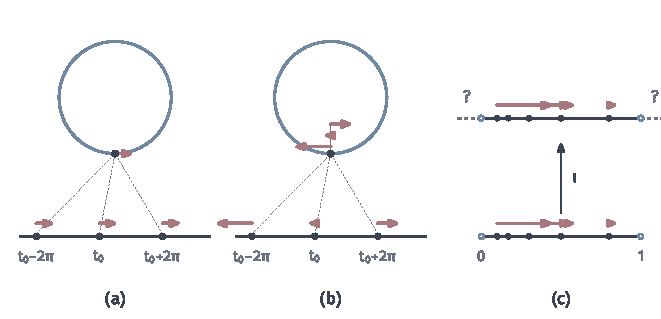
\includegraphics[width=112mm]{figures/04-spaces-measures-and-geometry/04-manifolds/matplotlib/mmaps-field-conflict/figure.pdf}
  \caption{逐点推送向量场。(a)$\frac{\mathrm d}{\mathrm dt}$在$E$的三个原像$t_0,t_0\pm2\pi$（$t_0=-\pi/2$）处推送结果一致。(b)$t\frac{\mathrm d}{\mathrm dt}$的三个推送结果不同；它们本来都在$E(t_0)$处，为看清而沿法向错开。箭头长度与$t$成正比。(c)包含映射$\iota$与场$\frac1t\frac{\mathrm d}{\mathrm dt}$：区间外没有原像（虚线），靠近$0$时箭头无限变长。}
  \label{fig:mmaps-field-conflict}
\end{BookInlineFigure}

\paragraph{$F$相关的向量场}
既然一般得不到目标上的向量场，就把问题反过来问：给定两侧的向量场，它们和$F$是否协调？这个提法不要求$F$单射或满射。

\begin{definition}[$F$相关]
\label{def:mmaps-f-related}
设$F:M\to N$光滑，$X\in\mathfrak X(M)$，$Y\in\mathfrak X(N)$。若对每个$p\in M$都有
\begin{equation}
\mathrm dF_p(X_p)=Y_{F(p)},
\label{eq:mmaps-f-related}
\end{equation}
则称$X$与$Y$是\term{$F$相关}（$F$-related）的。
\end{definition}

上面的例子中，$\frac{\mathrm d}{\mathrm dt}$与$\partial_\theta$是$E$相关的，而$t\frac{\mathrm d}{\mathrm dt}$不与$S^1$上任何向量场$E$相关。多个原像并不妨碍$F$相关，只要它们给出同一个值。

投影上有一个不平凡的例子。设$X$是球面的旋转场，在北极图中分量为$(-u_2,u_1)$；$Y$是平面上的旋转场，分量为$(-y_2,y_1)$。验证$p$和$q$两个原像，$p$处$\bm u=(0,3)$，$q$处$\bm u=(0,\tfrac13)$，分别代入
\[
\begin{aligned}
\operatorname{diag}(0.2,-0.16)\,(-3,\ 0)^\top&=(-0.6,\ 0)^\top,\\
\operatorname{diag}(1.8,1.44)\,(-\tfrac13,\ 0)^\top&=(-0.6,\ 0)^\top .
\end{aligned}
\]
两个结果相同，都等于$Y$在$(0,0.6)$处的值$(-0.6,0)$。这不是巧合：先转再投影等于先投影再转，$\pi$把球面上绕竖直轴的旋转变成平面上的旋转。

$F$相关还可以用向量场对函数的作用来刻画。这个刻画不涉及坐标，并且只用到向量场的代数作用，后面处理Lie括号时很方便。

\begin{lemma}[$F$相关的函数刻画]
\label{lem:mmaps-f-related-functions}
$X$与$Y$是$F$相关的，当且仅当对$N$的每个开子集$W$和每个$g\in C^\infty(W)$，在$F^{-1}(W)$上都有
\begin{equation}
X(g\circ F)=(Yg)\circ F .
\label{eq:mmaps-f-related-functions}
\end{equation}
\end{lemma}

\begin{proof}
在$p\in F^{-1}(W)$处，由链式法则\eqref{eq:mmaps-chain-rule}，
\[
X_p(g\circ F)=\mathrm d(g\circ F)_p(X_p)=\mathrm dg_{F(p)}\bigl(\mathrm dF_p(X_p)\bigr).
\]
而右端的$(Yg)(F(p))=\mathrm dg_{F(p)}(Y_{F(p)})$。若$X,Y$是$F$相关的，两者相等。

反过来，设两式对所有$g$相等。取$g$为$F(p)$附近图中的坐标函数$y_k$，$\mathrm dy_k$读出的是第$k$个分量，所以$\mathrm dF_p(X_p)$与$Y_{F(p)}$的第$k$个分量相等。对所有$k$成立，二者相等。
\end{proof}

用投影检验这个等式。取$g(\bm y)=y_2$，平面旋转场作用于它，$Yg=y_1$，于是右端的$(Yg)\circ\pi$是球面上的函数$y_1$。左端$g\circ\pi$是球面上的函数$y_2$，球面旋转场的速度是$(-y_2,y_1,0)$，所以$X(y_2)=y_1$，两端相等。

\begin{theorem}[$F$相关与Lie括号相容]
\label{thm:mmaps-f-related-bracket}
若$X_1$与$Y_1$、$X_2$与$Y_2$分别是$F$相关的，则$[X_1,X_2]$与$[Y_1,Y_2]$也是$F$相关的。
\end{theorem}

\begin{proof}
任取开集$W\subseteq N$与$g\in C^\infty(W)$。由引理~\ref{lem:mmaps-f-related-functions}，
\[
X_2(g\circ F)=(Y_2g)\circ F .
\]
两边再作用$X_1$，并对函数$Y_2g$用同一个引理，得到
\[
X_1X_2(g\circ F)=X_1\bigl((Y_2g)\circ F\bigr)=(Y_1Y_2g)\circ F .
\]
交换下标，得到另一个次序的等式，两式相减，
\[
[X_1,X_2](g\circ F)=([Y_1,Y_2]g)\circ F .
\]
再用一次引理的充分性，定理得证。
\end{proof}

用一个能手算的例子看定理在说什么。令$F:\mathbb R^2\to\mathbb R^2$，$F(x,y)=(x,\ y+x^2)$，目标的坐标记为$(a,b)$，Jacobian矩阵为
\[
\bm J_F=\begin{bmatrix}1&0\\2x&1\end{bmatrix}.
\]
取$X_1=\partial_x$，$X_2=x\,\partial_y$。逐列推送，再用$a=x$改写，得到与它们$F$相关的场：
\[
Y_1=\partial_a+2a\,\partial_b,\qquad Y_2=a\,\partial_b .
\]

分别计算两侧的括号。左侧只有$X_2$的系数依赖$x$，所以$[X_1,X_2]=\partial_y$，它的推送由$\bm J_F$的第二列给出，是$(0,1)^\top$，即$\partial_b$。右侧$Y_1$作用于$Y_2$的系数$a$得$1$，而$Y_2$作用于$Y_1$的系数$2a$得$0$，所以$[Y_1,Y_2]=\partial_b$，与推送结果相同。

\paragraph{双向光滑的双射}
若$F$是双射，每点恰有一个原像，上面的冲突和缺失都不会出现。若逆映射也光滑，推送所得的场还是光滑的。这类映射在第~\ref{chap:manifold-relations}章称为微分同胚，这里先说明它对向量场的作用。

\begin{theorem}[向量场的推送]
\label{thm:mmaps-pushforward-field}
设$F:M\to N$是光滑双射，且逆映射$F^{-1}$也光滑。对$X\in\mathfrak X(M)$，令
\begin{equation}
(F_*X)_q=\mathrm dF_{F^{-1}(q)}\bigl(X_{F^{-1}(q)}\bigr),\qquad q\in N .
\label{eq:mmaps-pushforward-field}
\end{equation}
则$F_*X$是$N$上的光滑向量场，并且是唯一与$X$为$F$相关的向量场。
\end{theorem}

\begin{proof}
$F$是双射，每个$q$有唯一原像，所以$F_*X$是良定义的向量场，并且按构造与$X$为$F$相关。任何与$X$为$F$相关的$Y$在$q=F(p)$处都必须等于$\mathrm dF_p(X_p)$，唯一性随之成立。

光滑性在坐标中检查。记$\hat X$为$X$的分量，在$q$附近的一对图中，$F_*X$的分量是
\[
\bm y\mapsto\bm J_{\hat F}\bigl(\widehat{F^{-1}}(\bm y)\bigr)\,\hat X\bigl(\widehat{F^{-1}}(\bm y)\bigr).
\]
$\widehat{F^{-1}}$光滑，$\bm J_{\hat F}$的元素与$\hat X$光滑，它们的复合与乘积仍光滑。
\end{proof}

逆映射光滑这个条件不能省。$F(x)=x^3$是$\mathbb R$到自身的光滑双射，它的逆映射$x^{1/3}$在原点不可微。推送$\frac{\mathrm d}{\mathrm dx}$，每点$x$处得到$3x^2\frac{\mathrm d}{\mathrm dy}$，用$x=y^{1/3}$写成目标坐标，
\[
(F_*X)_y=3y^{2/3}\,\frac{\mathrm d}{\mathrm dy}.
\]
分量$3y^{2/3}$在原点连续但有尖点，所以结果不光滑，见图~\ref{fig:mmaps-cube-field}。

\begin{BookInlineFigure}
  \centering
  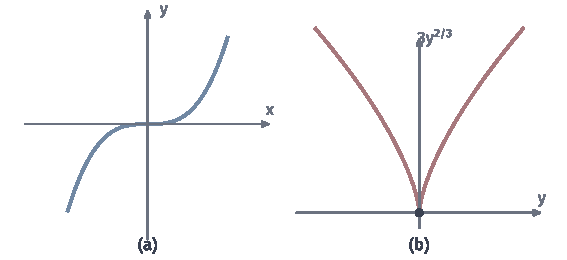
\includegraphics[width=96mm]{figures/04-spaces-measures-and-geometry/04-manifolds/matplotlib/mmaps-cube-field/figure.pdf}
  \caption{逆映射不光滑时的推送。(a)$F(x)=x^3$是光滑双射，在原点斜率为零。(b)$\frac{\mathrm d}{\mathrm dx}$的推送分量$3y^{2/3}$在$y=0$处出现尖点。}
  \label{fig:mmaps-cube-field}
\end{BookInlineFigure}

旋转$R_\theta$满足定理的条件，逆映射是$R_{-\theta}$。限制在$S^2\setminus\{N\}$上，北极图中$(R_\theta)_*X$的分量由式~\eqref{eq:mmaps-pushforward-field}给出：
\[
\bm u'\mapsto\bm R(\theta)\,\hat X\bigl(\bm R(-\theta)\bm u'\bigr).
\]

先取球面的旋转场，$\hat X(\bm u)=\bm R(\tfrac\pi2)\bm u$。平面旋转彼此可交换，三个旋转矩阵的转角相加，于是
\[
\bm R(\theta)\bm R(\tfrac\pi2)\bm R(-\theta)\bm u'=\bm R(\tfrac\pi2)\bm u'.
\]
旋转场被推送为自身：绕竖直轴转动，不改变绕竖直轴转动的速度场。

再取常分量场$\partial_{u_1}$，$\hat X=\bm e_1$。代入后结果不依赖$\bm u'$，
\[
\bm R(\theta)\bm e_1=(\cos\theta,\ \sin\theta)^\top ,
\]
也就是
\[
(R_\theta)_*\partial_{u_1}=\cos\theta\,\partial_{u_1}+\sin\theta\,\partial_{u_2}.
\]
整片箭头跟着转了$\theta$，见图~\ref{fig:mmaps-rotation-field-push}。

\begin{BookInlineFigure}
  \centering
  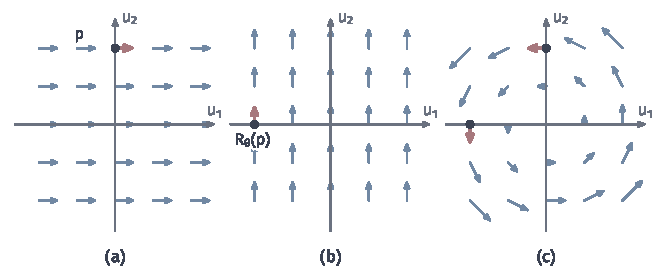
\includegraphics[width=112mm]{figures/04-spaces-measures-and-geometry/04-manifolds/matplotlib/mmaps-rotation-field-push/figure.pdf}
  \caption{旋转$R_\theta$（$\theta=\pi/2$）在北极图中推送向量场。(a)常分量场$\partial_{u_1}$（蓝），红箭头是$p$处的值。(b)推送结果$\partial_{u_2}$，$p$处的红箭头被送到$R_\theta(p)$处。(c)旋转场$(-u_2,u_1)$，推送后不变，红箭头是$p$与$R_\theta(p)$处的值，箭头长度按$0.28$缩放。}
  \label{fig:mmaps-rotation-field-push}
\end{BookInlineFigure}

\section{协向量的拉回}
\label{sec:mmaps-pullback}

切向量随映射向前推，从$p$处送到$F(p)$处。余切向量是对切向量的读数，它的换算方向恰好相反：如果已经知道怎样在$F(p)$处读数，就可以先把$p$处的切向量推过去，再在那里读数，这样得到的是$p$处的一个读数。本节把这个想法写成定义，并说明方向相反带来的好处。

\paragraph{逐点的拉回}
设$F:M\to N$光滑，$p\in M$，$\omega\in T^*_{F(p)}N$。对$\bm v\in T_pM$，$\mathrm dF_p(\bm v)$属于$T_{F(p)}N$，可以被$\omega$读取。

\begin{definition}[余切向量的拉回]
\label{def:mmaps-covector-pullback}
$\mathrm dF_p$的对偶映射
\[
(\mathrm dF_p)^*:T^*_{F(p)}N\to T^*_pM,\qquad
\bigl((\mathrm dF_p)^*\omega\bigr)(\bm v)=\omega\bigl(\mathrm dF_p(\bm v)\bigr)
\]
称为$F$在$p$处的余切映射，$(\mathrm dF_p)^*\omega$称为$\omega$的\term{拉回}（pullback）。
\end{definition}

右端对$\bm v$线性，所以$(\mathrm dF_p)^*\omega$确实是$p$处的余切向量；它对$\omega$也线性。在坐标中，设$\omega=\sum_kb_k\,\mathrm dy_k|_{F(p)}$，$\bm J=\bm J_{\hat F}(\varphi(p))$。把$(\mathrm dF_p)^*\omega$作用在$\partial_j|_p$上，由式\eqref{eq:mmaps-differential-basis}得到它的第$j$个系数$\sum_kb_k\,\partial\hat F_k/\partial x_j$。写成列向量，
\begin{equation}
\bm a=\bm J^\top\bm b .
\label{eq:mmaps-pullback-coordinates}
\end{equation}
切向量的分量用$\bm J$从$M$推到$N$，余切向量的系数用$\bm J^\top$从$N$拉回$M$，两个方向相反。

\paragraph{协向量场的拉回总有定义}
对$N$上的协向量场$\omega$，在每个$p\in M$处拉回$F(p)$处的值，得到$M$上的协向量场
\[
(F^*\omega)_p=(\mathrm dF_p)^*\bigl(\omega_{F(p)}\bigr),\qquad p\in M .
\]
这里每个$p$只需要一个值$\omega_{F(p)}$，它总是存在且唯一。所以向量场推送时遇到的两类困难都不出现：多个原像只是各自拉回同一个值，没有原像的点在$M$中根本不出现。在坐标中，$F^*\omega$的系数是$\bm J_{\hat F}(\bm x)^\top\hat{\bm b}(\hat F(\bm x))$，由光滑函数复合、相乘得到，所以$\omega$光滑时$F^*\omega$也光滑。拉回对任何光滑映射都适用，不需要$F$可逆。

\paragraph{运算规则}
拉回与函数、复合和微分的关系可以归结为三条规则。

\begin{theorem}[拉回的运算规则]
\label{thm:mmaps-pullback-rules}
设$F:M\to N$与$G:N\to P$光滑，$\omega$是$N$上的光滑协向量场，$g,f\in C^\infty(N)$。则
\begin{enumerate}
\item $F^*(g\,\omega)=(g\circ F)\,F^*\omega$；
\item $(G\circ F)^*=F^*\circ G^*$；
\item $F^*(\mathrm df)=\mathrm d(f\circ F)$。
\end{enumerate}
\end{theorem}

\begin{proof}
第一条：在$p$处，$g\,\omega$的值是$g(F(p))\,\omega_{F(p)}$，对偶映射线性，系数$g(F(p))$直接提出。第二条：由链式法则，$\mathrm d(G\circ F)_p=\mathrm dG_{F(p)}\circ\mathrm dF_p$；对偶映射交换复合次序，$(\mathrm d(G\circ F)_p)^*=(\mathrm dF_p)^*\circ(\mathrm dG_{F(p)})^*$。第三条：对$\bm v\in T_pM$，
\[
\bigl(F^*\mathrm df\bigr)_p(\bm v)=\mathrm df_{F(p)}\bigl(\mathrm dF_p(\bm v)\bigr)=\mathrm d(f\circ F)_p(\bm v),
\]
最后一步是链式法则应用于$f\circ F$。
\end{proof}

第三条说明“先微分再拉回”与“先复合再微分”给出同一个结果。复合次序在第二条中反过来：先作用$F$再作用$G$的映射，拉回时先用$G^*$再用$F^*$。这与切向量的推送$\mathrm d(G\circ F)=\mathrm dG\circ\mathrm dF$方向相反，是对偶映射的一般性质。

\paragraph{例子：圆周上的角度读数}
圆周上的两张角度图相差常数平移，所以$\mathrm d\theta_1$与$\mathrm d\theta_2$在重叠处相等，拼成整个圆周上的光滑协向量场，记为$\mathrm d\theta$。注意它不是某个全局光滑函数的微分，因为圆周上没有处处光滑的全局角度函数，记号只表示它在每张图中都是坐标函数的微分。

用$E(t)=(\cos t,\sin t)$拉回：$E$在角度图中的坐标表示是$t\mapsto t+c$，导数为$1$，由式\eqref{eq:mmaps-pullback-coordinates}，$E^*(\mathrm d\theta)=\mathrm dt$。这里$E$不是单射，每个圆周上的点有无穷多个原像，拉回照样良定义。这一计算也证实了上一段的断言：若$\mathrm d\theta=\mathrm df$对某个$f\in C^\infty(S^1)$成立，则由第三条规则$\mathrm d(f\circ E)=E^*\mathrm d\theta=\mathrm dt$，于是$f(E(t))=t+c$；但$f\circ E$以$2\pi$为周期，矛盾。与上一节对比，$\mathbb R$上的向量场$t\frac{\mathrm d}{\mathrm dt}$无法推送到圆周，而圆周上的协向量场总能拉回$\mathbb R$。

\paragraph{例子：旋转下的高度读数}
由运算规则的第三条，$R_\theta^*(\mathrm dh)=\mathrm d(h\circ R_\theta)=\mathrm dh$，因为旋转不改变高度。这与上一节在$p=(0,\tfrac35,\tfrac45)$处的矩阵计算是同一件事：那里用行向量左乘$\bm R(\theta)$，正是式\eqref{eq:mmaps-pullback-coordinates}的转置形式。用拉回的语言，计算不需要逐点核对，直接由函数的不变性得出。

\paragraph{向更一般对象的推广}
本节只拉回了余切向量，即对单个切向量的线性读数。同样的思路可以用于同时读取多个切向量的多重线性读数，例如面积元和体积元，其中最重要的是交替的情形，即微分形式。它们的拉回、外微分及与积分的关系，在第~\ref{chap:manifold-calculus}章定义交替形式之后建立；黎曼度量作为对两个切向量的对称读数，其拉回在第~\ref{chap:riemannian-geometry}章用于定义等距映射。

\section{本章小结}
\label{sec:mmaps-summary}

本章开头问：给定流形之间的映射，它怎样对应点，又怎样改变点处的方向和读数？对点而言，光滑映射由两侧坐标图中的坐标表示判断，换用相容的图不改变结论。同一个坐标公式可能描述两件事：同一点在两张图中的记录之间的换算，或者把点实际送到另一个点；前者是恒等映射的坐标表示，后者才移动了点。曲线和实值函数都是光滑映射的特例。

对方向而言，映射的微分$\mathrm dF_p:T_pM\to T_{F(p)}N$把经过$p$的曲线速度推送为经过$F(p)$的曲线速度，在坐标基下的矩阵是坐标表示的Jacobian矩阵；边界点处用光滑延拓的Jacobian矩阵，结果与延拓无关。链式法则$\mathrm d(G\circ F)_p=\mathrm dG_{F(p)}\circ\mathrm dF_p$成立，秩不依赖图，实值函数的微分与第~\ref{chap:manifold-basics}章的余切向量$\mathrm df_p$一致。

对整个向量场逐点推送时，不同原像可能给出同一点处相互冲突的向量，像以外的点没有值，所以一般映射不能把向量场推送成目标上的向量场。能做的是判断两侧的场是否$F$相关，它等价于$X(g\circ F)=(Yg)\circ F$，并与Lie括号相容。若映射是光滑双射且逆映射光滑，推送得到唯一的光滑向量场；逆映射不光滑时，例如$x\mapsto x^3$，推送结果可能不光滑。

对读数而言，余切向量沿相反方向拉回：$(\mathrm dF_p)^*\omega=\omega\circ\mathrm dF_p$，坐标中由Jacobian矩阵的转置给出。协向量场的拉回对任何光滑映射都有定义，因为每个原像点只需要一个目标值；它满足$(G\circ F)^*=F^*\circ G^*$与$F^*(\mathrm df)=\mathrm d(f\circ F)$。推送与拉回的方向不同、作用对象不同，所需的条件也不同。

这些都是映射的局部操作。微分可逆、单射或满射分别说明映射在一点附近保留或覆盖了多少方向，但不能单独决定两个流形整体上是否等价，或一个流形的像能否成为子流形。第~\ref{chap:manifold-relations}章在本章的微分与秩的基础上，加入可逆性与拓扑条件来回答这些问题。

